\documentclass[letterpaper,12pt]{article}
\usepackage{tabularx} % extra features for tabular environment
\usepackage{amsmath}  % improve maths presentation
\usepackage{amssymb} % maths symbols
\usepackage{graphicx} % takes care of graphic including machinery
\usepackage[margin=0.95in,letterpaper]{geometry} % decreases margins
\usepackage{cite} % takes care of citations
\usepackage[titletoc,title]{appendix} % takes care of appendices
\usepackage{listings} % code representation
\usepackage{pdflscape}
\usepackage{csquotes} % for quoting existing work
\usepackage{color} % defines colours for code listings
\usepackage{comment} % allows for block of comments
\usepackage{gensymb} % degree symbol
\usepackage[table,xcdraw]{xcolor} % table colouring
\usepackage[cc]{titlepic}  % allows a pic to be included in the title page
\usepackage[final]{hyperref} % adds hyper links inside the generated pdf file
\usepackage{pdfpages} % include pdfs

% style code listings
\definecolor{codegreen}{rgb}{0,0.6,0}
\definecolor{codegray}{rgb}{0.5,0.5,0.5}
\definecolor{backcolour}{rgb}{0.95,0.95,0.92}
\lstdefinestyle{mystyle}{
    backgroundcolor=\color{backcolour},   
    commentstyle=\color{codegreen},
    keywordstyle=\color{blue},
    numberstyle=\tiny\color{codegray},
    basicstyle=\footnotesize,
    breakatwhitespace=false,         
    breaklines=true,                 
    captionpos=b,                    
    keepspaces=true,                 
    numbersep=5pt,                  
    showspaces=false,                
    showstringspaces=false,
    showtabs=false,                  
    tabsize=4
}
\lstset{style=mystyle}

\begin{document}

\title{
    CS5011 Artificial Intelligence Practice\\Assignment 4 Report\\
    \begin{large}
    University of St Andrews - School of Computer Science
    \end{large}
}
\titlepic{
\includegraphics[width=0.3\linewidth]{report/figures/st-andrews-logo.jpeg}}
\author{Student ID: 150014151}
\date{20th December, 2019}
\maketitle
\newpage

\tableofcontents
\newpage


% --------------------------------------- 1 - INTRODUCTION ------------------------------------------ 

\section{Introduction}
\label{sec:introduction}

The following requirements were attempted:
\begin{itemize}
    \item Basic Agent:
    \begin{itemize}
        \item Multilayer feedforward neural network.
        \item Data encoding and training/testing split.
        \item Grid search algorithm for determining optimal hyperparameters.
    \end{itemize}
    \item Intermediate Agent:
    \begin{itemize}
        \item CLI text-based interface.
    \end{itemize}
    \item Additional Features:
    \begin{itemize}
        \item Training result visualisation in plots and heatmaps.
    \end{itemize}
        
\end{itemize}

\subsection{Installation}

Create a virtual environment for the project and activate it:

\begin{lstlisting}
virtualenv ~/Environments/A4
source ~/Environments/A4/bin/activate
\end{lstlisting}

Once you have the virtual environment activated, \textit{cd} into the project directory and install the requirements needed to run the app:

\begin{lstlisting}
pip install -r requirements.txt
\end{lstlisting}

\subsection{Usage}

To compile the program, navigate to the \textit{A4src} directory and run the following command:

\begin{lstlisting}
python A4Main.py [-h] -a <AGENT> -c <CSV> [-g] [-d]
\end{lstlisting}

where:

\begin{itemize}
    \item \textit{AGENT} is the type of agent to run: \textit{[Bas, Int, Adv]}:
    \begin{itemize}
        \item \textit{Bas}: Train and test the neural network with the optimal parameters, or run the Grid Search algorithm to determine the optimal parameters.
        \item \textit{Int}: CLI text-based application to submit a new ticket and predict to which response team it should go.
        \item \textit{Adv}: todo.
    \end{itemize}
    \item \textit{CSV} is the CSV file containing the data used to train/test the data.
    \item \textit{-g}: flag set to run the grid search algorithm.
    \item \textit{-d}: flag set to enter debug mode, printing more statements to the command line.
    \item \textit{-h}: flag for help on how to use the agent.
\end{itemize}

\paragraph{Examples}

Here are a few examples that can be used to run the program:

\begin{itemize}
    \item ``\textit{python A4Main.py -a Bas -c tickets -d}'' to train/test the neural network.
    \item ``\textit{python A4Main.py -a Bas -c tickets -g}'' to run the grid search algorithm.
    \item ``\textit{python A4Main.py -a Int -c tickets}'' to submit a new ticket through the CLI text-based interface
    \item ``\textit{python A4Main.py -h}'' for help on how to run the agent.
\end{itemize}

\subsection{Tools Used}

\begin{itemize}
    \item Scikit\footnote{Scikit: \url{https://scikit-learn.org}} and related Python libraries (e.g. NumPy\footnote{NumPy: \url{https://numpy.org/}}, Pandas\footnote{Pandas: \url{https://pandas.pydata.org/}}, Matplotlib\footnote{Matplotlib: \url{https://matplotlib.org/}}).
    \item PyCharm\footnote{PyCharm: \url{https://www.jetbrains.com/pycharm/}}: an IDE developed by JetBrains to write Python code with support for some of the above libraries.
    \item Git and GitHub: to back and version control the code.
    \item PEP8\footnote{PEP8: \url{https://www.python.org/dev/peps/pep-0008/}} coding guidelines and docstring followed throughout the entire code.
\end{itemize}

% -------------------------- 2 - DESIGN - IMPLEMENTATION - EVALUATION -------------------------------

\clearpage
\section{Design, Implementation \& Evaluation}
\label{sec:design-implementation-evaluation}

\subsection{Design: PEAS Model}

This section defines the PEAS model for a ticketing routing-based agent that uses a multilayer feedforward neural network in order to ultimately learn how to make smart predictions for the appropriate response team of future tickets.

\paragraph{Performance measure}\label{sec:performance-measures} The basic agent can be evaluated by the efficiency of the training step based on the number of epochs required to train to a certain target error, and the testing accuracy using a confusion matrix. The intermediate agent can be assessed by the number of questions to make a prediction and their correctness can also be measured.

\paragraph{Environment} This is a single-agent and fully-observable environment represented by a neural network and the text-based interface used to interact with a user logging a new ticket. Additionally, it can be said that the basic agent environment is deterministic (the next state is determined by the current state and the action executed) and stochastic for the intermediate agent (user input is unknown), according to the definitions set by Russell \& Norvig in \textit{Artificial intelligence: a modern approach} \cite{russell2016artificial}.

\paragraph{Actuators} The agent may accept input and target data it can learn from by backpropagating the calculated error between the input and target data in order to adjust the weights of the neural network (also known as Stochastic Gradient Descent). It may also predict an output based on unseen data.

\paragraph{Sensors} The basic agent is always aware of the environment and can calculate feedback error based on input and target data, while the intermediate agent can receive responses to questions by interacting with a human user.

% ----------------------------------

\subsection{Implementation}

\subsubsection{Project Structure}

The project is divided in three main sections:

\begin{itemize}
    \item The \textit{agents} module, containing functions to implement the execution of flow of each agent.
    \item The \textit{neural\_network} module, which contains classes to create and manipulate a multilayered perceptron, a data encoder/processor and the grid search algorithm.
    \item The \textit{main} section, containing the program's entry point \textit{A4Main.py} for parsing the command line arguments, global configuration settings in \textit{config.py} and printing methods in \textit{helpers.py}.
\end{itemize}

The \textit{data} directory stores the CSV data, the \textit{neural\_networks} directory the trained neural nets in \textit{``*.joblib''} format, and the \textit{results} directory the output of the grid search algorithm.

% ----------------------------------

\subsubsection{Neural Network Training \& Testing (Basic Agent)}
\label{sec:basic-agent}

The basic agent takes a CSV file as input to be used for training and testing. It instantiates the custom \textit{DataProcessor} class containing functions for parsing the CSV file (retrieving tags and categories), splitting the data between inputs and targets, and encoding/decoding it. The input data is encoded in either 0s or 1s, while the target data is encoded using one-hot encoding. Figure \ref{fig:data_encoding} depicts how the data is split and encoded.

\begin{figure}[h] 
\centerline{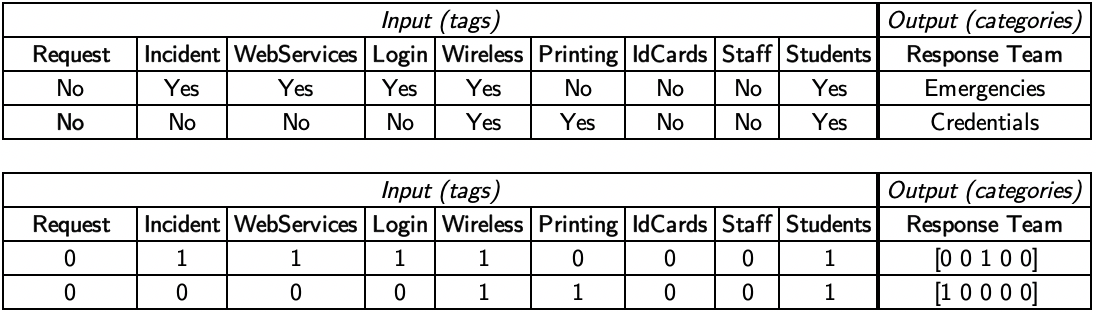
\includegraphics[width=\textwidth]{report/figures/data_encoding.png}}
\caption{\label{fig:data_encoding}At the top, the decoded data; at the bottom, the encoded data.}
\end{figure}

The data must be fed to the neural network in binary form. One-hot encoding is therefore chosen as it suits the sparse representation of the data, which is made up of only five target categories. Only a single digit may have the value 1 in one-hot encoding, while the others remain at value 0 \cite{lec16}. The one-hot encodings of the target categories can be seen in Figure \ref{fig:one_hot_encoding}.

\begin{figure}[h] 
\centerline{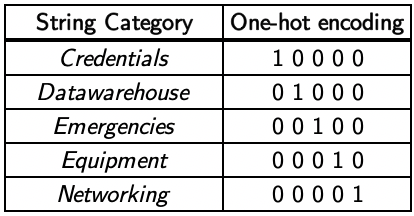
\includegraphics[width=0.4\textwidth]{report/figures/one_hot_encoding.png}}
\caption{\label{fig:one_hot_encoding}One-hot encoding of the categories.}
\end{figure}

Once the data is encoded, an instance of the custom \textit{MultiLayerPerceptron} class is created, containing functions to split the training/testing data, training \& testing the neural network, displaying results and saving the network with the trained weights. The class uses \textit{Scikit}'s \textit{MLPClassifier}\footnote{Scikit MLPClassifier: \url{https://scikit-learn.org/stable/modules/generated/sklearn.neural_network.MLPClassifier.html}} to implement the neural network and is instantiated with optimal hyperparameters determined in Section \ref{sec:optimal-hyperparams} for the neural network, which can be overwritten when creating a new \textit{MultiLayerPerceptron} (see Listing below).

\begin{lstlisting}[language=Python]
class MultiLayerPerceptron:
    def __init__(self, name, input_data, target_data, hidden_layers_size=(15,), solver="adam", activation_function="logistic", learning_rate_init=0.6, momentum=0.9, optimisation_tolerance=0.0001, num_iterations_no_change=1000, max_iterations=10000, verbose=config.debug):
\end{lstlisting}

An 80\%/20\% split is used for the training/testing data sets, with equal category distribution maintained between the training and testings sets, which is ensured through the use of the \textit{stratify} option in Scikit's \textit{train\_test\_split} function\footnote{Scikit train\_test\_split: \url{https://scikit-learn.org/stable/modules/generated/sklearn.model_selection.train_test_split.html}}. Because the data has 250 entries (including 50 for each of five outputs), the testing set will have 10 entries for each of the five categories.\\

The actual training is carried out using the \textit{fit} function, with the error loss plotted with regards to the number of epochs; while the testing is performed using the \textit{predict} and \textit{predict\_proba} functions and its accuracy visualised with a confusion matrix (counting the number of true positives/negatives and false positives/negatives) in a heatmap. These results can be seen in Section \ref{sec:eval-errorloss-cm}.

% ----------------------------------

\subsubsection{CLI-Based Ticketing-Routing Agent (Intermediate Agent)}

The intermediate agent is built on a CLI\footnote{Command Line Interface} as an interactive text-based application allowing a human user to submit a new ticket. The agent records the \textit{``Yes''}/\textit{``No''} answers to each tag to create a new ticket, which is then used to as input to the previously trained neural network to make a prediction. The neural net is loaded using \textit{joblib} and tested using the \textit{predict} and \textit{predict\_proba} function.\\

To avoid the repetitive task of answering all questions, the agent makes early predictions after the third, fifth and seventh questions. The prediction is made by filling out the missing fields in the ticket with the most common value (\textit{mode}) in the original CSV data.\\

After an early prediction is made, the user can state whether he is happy with the result or not. If he is not, the agent asks more questions until the next early prediction or until all questions have been answered. Finally, if the user is not happy with the final prediction, he can specify the desired response team to send the ticket to (only if he has answered all questions and entered \textit{``No''} to every early prediction). This information is added to the end of a copy of the original CSV data file that is used to re-train the neural network in a similar fashion mentioned in Section \ref{sec:basic-agent}. The newly trained network is then saved and used for future predictions.

% ----------------------------------

\subsubsection{Advanced}

todo


% ----------------------------------

\subsection{Evaluation}
\label{sec:evaluation}

\subsubsection{Optimal Hyperparameters}
\label{sec:optimal-hyperparams}

In order to find the optimal hyperparameters to train the neural network, a grid search algorithm is implemented. The algorithm exhaustively trains and tests the neural network with every combination from a pre-defined set of parameters and measures its accuracy. The parameters tested include the number of neurons in the hidden layer, the solver, the activation function, the learning rate, the momentum, the tolerance and the maximum number of iterations after which training stops if error does not improve by the tolerance. These can be found in the Listing below:

\begin{lstlisting}[language=Python]
grid_search_params = {
    `hidden_layer_sizes': [(3,), (5,), (7,), (9,), (15,), (25,)],
    `solver': ["sgd", "adam"],
    `activation': ["logistic", "relu", "tanh"],
    `learning_rate_init': [0.05, 0.1, 0.2, 0.4, 0.6, 0.8, 1.0],
    `momentum': [0.1, 0.3, 0.5, 0.7, 0.9],
    `tol': [1, 0.1, 0.01, 0.001, 0.0001],
    `n_iter_no_change': [100, 1000],
    `max_iter': [10000]  # Parameter not being tested.
}
\end{lstlisting}

Overall, 12,600 unique combinations of parameters were tested in 1h26m. From these tests, 14 combinations of hyperparameters with a +98\% mean accuracy (over 5 runs for even 80\%/20\% data splits) emerged as optimal, as depicted in Figure \ref{fig:gridsearch_results}. These optimal parameters can be found in Appendix \ref{sec:appendix-optimal-hyperparameters}.

\begin{figure}[h] 
\centerline{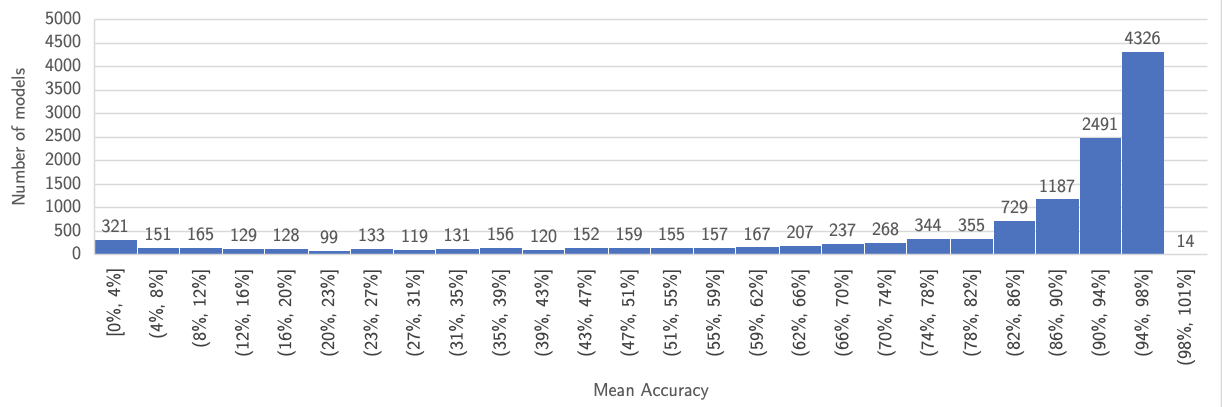
\includegraphics[width=\textwidth]{report/figures/gridsearch_results.png}}
\caption{\label{fig:gridsearch_results}14 best combinations of hyperparamaters.}
\end{figure}

It is interesting to note that over half of these tests result in accuracies range between [90\%-98\%[. This is likely due to the fact that there is very little data to begin with (only 250 entry points), meaning that unless the chosen hyperparameters are really poor (e.g. 3 hidden units with momentum 0.1 and tolerance 1, resulting in a mean accuracy of 5.5\%), the neural network will always train to an acceptable level. The lack of data is also convincing enough to avoid finding optimal general parameters through validation.

\subsubsection{Error Loss and Confusion Matrices}
\label{sec:eval-errorloss-cm}

Four optimal combinations of hyperparameters have been chosen for comparison, along with one poor set of hyperparameters to point out differences. These can be found in Table \ref{tab:nn_hyperparam_eval}.

\begin{table}[h]
\centering
\begin{tabular}{|c|c|c|c|c|c|c|c|}
\hline
\textbf{Activation}             & \textbf{\begin{tabular}[c]{@{}c@{}}Hidden\\ Neurons\end{tabular}} & \textbf{$\alpha$}          & \textbf{$\beta$}           & \textbf{\begin{tabular}[c]{@{}c@{}}N Iter \\ \\ No Change\end{tabular}} & \textbf{Solver}             & \textbf{Tol}                  & \textbf{\begin{tabular}[c]{@{}c@{}}Mean \\ \\ Accuracy\end{tabular}} \\ \hline
{\color[HTML]{036400} logistic} & {\color[HTML]{036400} (15,)}                                      & {\color[HTML]{036400} 0.6} & {\color[HTML]{036400} 0.9} & {\color[HTML]{036400} 1000}                                             & {\color[HTML]{036400} adam} & {\color[HTML]{036400} 0.0001} & {\color[HTML]{036400} 98.5\%}                                        \\ \hline
{\color[HTML]{009901} tanh}     & {\color[HTML]{009901} (5,)}                                       & {\color[HTML]{009901} 0.8} & {\color[HTML]{009901} 0.1} & {\color[HTML]{009901} 100}                                              & {\color[HTML]{009901} sgd}  & {\color[HTML]{009901} 0.0001} & {\color[HTML]{009901} 98.0\%}                                        \\ \hline
{\color[HTML]{009901} logistic} & {\color[HTML]{009901} (9,)}                                       & {\color[HTML]{009901} 0.2} & {\color[HTML]{009901} 0.9} & {\color[HTML]{009901} 1000}                                             & {\color[HTML]{009901} adam} & {\color[HTML]{009901} 0.1}    & {\color[HTML]{009901} 98.0\%}                                        \\ \hline
{\color[HTML]{009901} tanh}     & {\color[HTML]{009901} (25,)}                                      & {\color[HTML]{009901} 1}   & {\color[HTML]{009901} 0.1} & {\color[HTML]{009901} 1000}                                             & {\color[HTML]{009901} sgd}  & {\color[HTML]{009901} 0.001}  & {\color[HTML]{009901} 98.0\%}                                        \\ \hline
{\color[HTML]{CB0000} logistic} & {\color[HTML]{CB0000} (3,)}                                       & {\color[HTML]{CB0000} 1}   & {\color[HTML]{CB0000} 0.5} & {\color[HTML]{CB0000} 1000}                                             & {\color[HTML]{CB0000} adam} & {\color[HTML]{CB0000} 0.001}  & {\color[HTML]{CB0000} 38.0\%}                                        \\ \hline
\end{tabular}
\caption{The 5 neural network hyperparameters used for evaluation, including 4 optimal and 1 sub-optimal.}
\label{tab:nn_hyperparam_eval}
\end{table}

Plotting the error function with respect to the number of epochs required to reach the designated tolerance gives interesting insights about the training, as seen in Figure \ref{fig:error-loss-curve}. Indeed, the error loss curve is similar when using optimal parameters, quickly converging towards the desired error. A notable difference is the effect of a low momentum $\beta=0.1$ on the convergence speed, causing the light blue slope to reach the desired error more slowly than neural networks with high momentum. However, the actual difference between training with optimal parameters (accuracy $\geqslant$ 98\%) and sub-optimal parameters (accuracy = 38\%) is that the error loss curve is less smooth (small peaks can be seen across the curve, especially before epoch 50) due to the high learning rate and lack of neural units (data is under-fitted) and it characterised by multiple plateaus. Other cases of sub-optimal neural networks would cause ravines, which would be solved with a higher momentum, or will cause the neural network over-fit the data due to a high number of hidden neurons.

\begin{figure}[h] 
\centerline{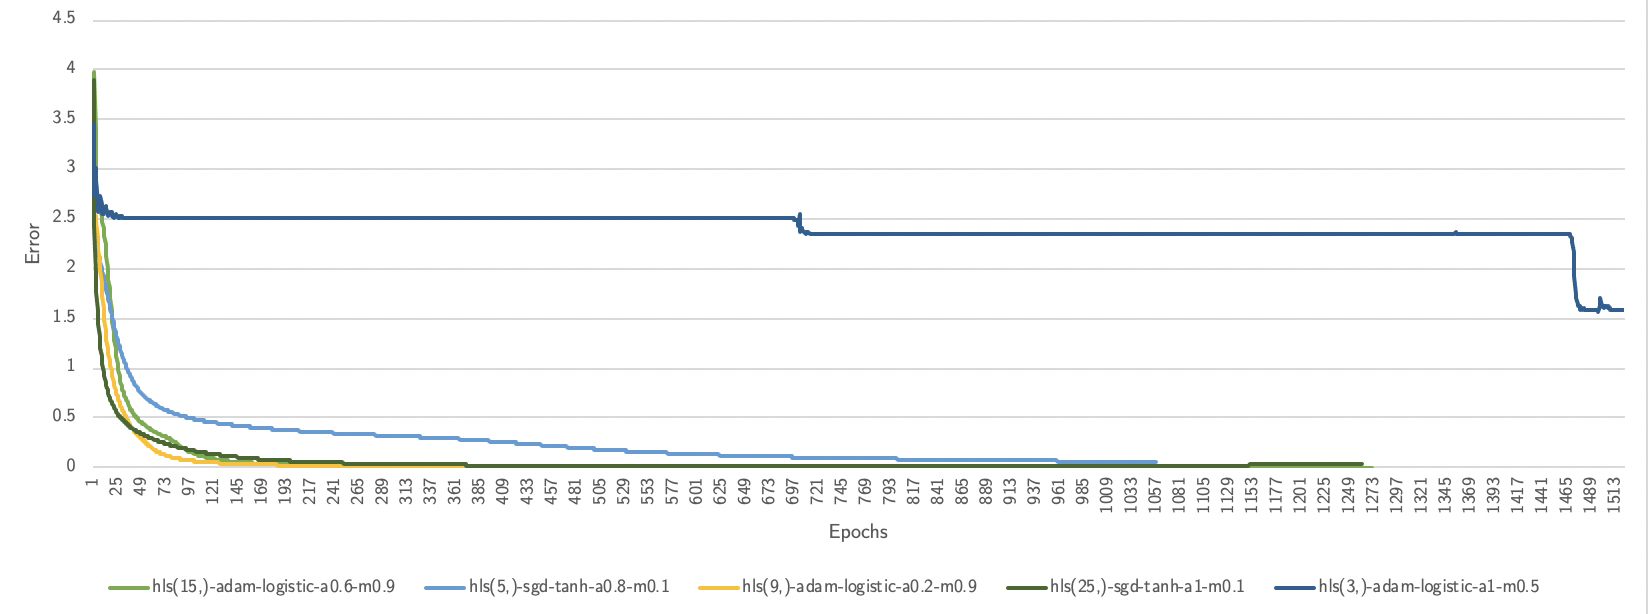
\includegraphics[width=\textwidth]{report/figures/error_loss_curve.png}}
\caption{\label{fig:error-loss-curve}Error loss.}
\end{figure}

Once the training is completed, an aggregated confusion matrix over five runs is calculated and plotted in a heatmap for each neural network. The results can be seen in Figure \ref{fig:confusion_matrices}.

\begin{figure}[h] 
\centerline{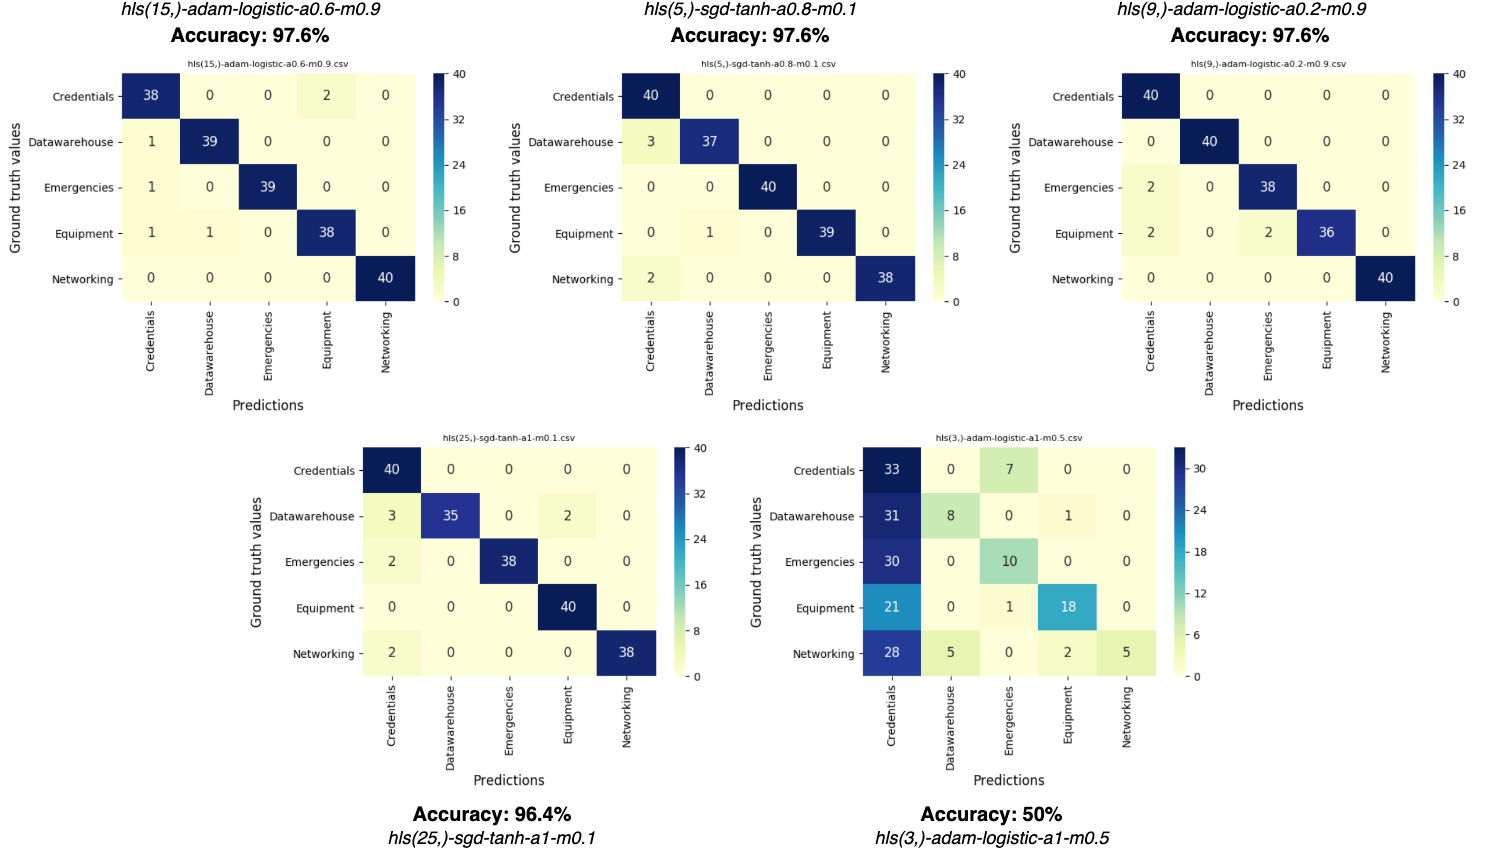
\includegraphics[width=1.1\textwidth]{report/figures/confusion_matrices.png}}
\caption{\label{fig:confusion_matrices}CM.}
\end{figure}

\subsubsection{Ticketing Routing Agent}

A demo is attached in the appendix.

When the user creates a new ticket and suggest which team to respond to, the neural network is retrained. However, answering the questions the same way does not predict the 

This may be due to the fact that a single row is not enough to shift the weights between the neurons enough for the desired output. Perhaps if a dozen users all suggested the same correction to the agent, then the weights would change enough to allow the suggested team to be predicted.

% retraining with new row doesn;t change outcome, need more users to request change

\textit{Design, Implementation \& Evaluation Section word count: \underline{XXXX}}

% -------------------------------------- 3 - TEST SUMMARY ------------------------------------------ 
\section{Test Summary}
\label{sec:test-summary}

todo


% -------------------------------------- APPENDICES ------------------------------------------ 
\begin{appendices}

\clearpage
\bibliographystyle{plain}
\bibliography{bibliography}

% ------------------------

\clearpage
\section{Project File Structure}
\label{sec:appendix-project-file-structure}

todo

% ------------------------

\clearpage
\section{Optimal Hyperparameters}
\label{sec:appendix-optimal-hyperparameters}

\begin{landscape}
\begin{table}[]
\begin{tabular}{|c|c|c|c|c|c|c|c|c|}
\hline
\textbf{Activation} & \textbf{\begin{tabular}[c]{@{}c@{}}Hidden \\ \\ Layer \\ \\ Size\end{tabular}} & \textbf{\begin{tabular}[c]{@{}c@{}}Learning \\ \\ Rate\end{tabular}} & \textbf{Momentum} & \textbf{\begin{tabular}[c]{@{}c@{}}N Iter \\ \\ No Change\end{tabular}} & \textbf{Solver} & \textbf{Tolerance} & \textbf{\begin{tabular}[c]{@{}c@{}}Mean \\ \\ Accuracy\end{tabular}} & \textbf{\begin{tabular}[c]{@{}c@{}}Mean \\ \\ Fit Time \\ \\ (seconds)\end{tabular}} \\ \hline
logistic            & (15,)                                                                          & 0.6                                                                  & 0.9               & 1000                                                                    & adam            & 0.0001             & 98.5\%                                                               & 1.61                                                                                 \\ \hline
tanh                & (5,)                                                                           & 0.4                                                                  & 0.7               & 100                                                                     & sgd             & 0.0001             & 98.0\%                                                               & 0.51                                                                                 \\ \hline
tanh                & (5,)                                                                           & 0.8                                                                  & 0.1               & 100                                                                     & sgd             & 0.0001             & 98.0\%                                                               & 0.61                                                                                 \\ \hline
tanh                & (5,)                                                                           & 1                                                                    & 0.3               & 1000                                                                    & sgd             & 1                  & 98.0\%                                                               & 0.77                                                                                 \\ \hline
logistic            & (9,)                                                                           & 0.2                                                                  & 0.9               & 1000                                                                    & adam            & 0.1                & 98.0\%                                                               & 0.78                                                                                 \\ \hline
tanh                & (5,)                                                                           & 0.05                                                                 & 0.9               & 1000                                                                    & adam            & 0.1                & 98.0\%                                                               & 0.80                                                                                 \\ \hline
tanh                & (15,)                                                                          & 0.8                                                                  & 0.7               & 1000                                                                    & sgd             & 0.01               & 98.0\%                                                               & 0.81                                                                                 \\ \hline
tanh                & (5,)                                                                           & 1                                                                    & 0.7               & 1000                                                                    & sgd             & 0.001              & 98.0\%                                                               & 0.86                                                                                 \\ \hline
tanh                & (9,)                                                                           & 0.2                                                                  & 0.3               & 1000                                                                    & adam            & 0.1                & 98.0\%                                                               & 0.92                                                                                 \\ \hline
tanh                & (25,)                                                                          & 0.4                                                                  & 0.9               & 1000                                                                    & sgd             & 1                  & 98.0\%                                                               & 0.93                                                                                 \\ \hline
tanh                & (5,)                                                                           & 0.05                                                                 & 0.9               & 1000                                                                    & sgd             & 0.001              & 98.0\%                                                               & 0.93                                                                                 \\ \hline
logistic            & (25,)                                                                          & 0.4                                                                  & 0.9               & 1000                                                                    & adam            & 0.01               & 98.0\%                                                               & 0.95                                                                                 \\ \hline
tanh                & (25,)                                                                          & 1                                                                    & 0.1               & 1000                                                                    & sgd             & 0.001              & 98.0\%                                                               & 1.12                                                                                 \\ \hline
logistic            & (9,)                                                                           & 0.4                                                                  & 0.3               & 1000                                                                    & sgd             & 0.0001             & 98.0\%                                                               & 1.65                                                                                 \\ \hline
\end{tabular}
\caption{The 14 optimal hyperparameters founds after the grid search algorithm on 12,600 combinations.}
\label{tab:optimal-hyperparameters}
\end{table}
\end{landscape}

% ------------------------

\clearpage
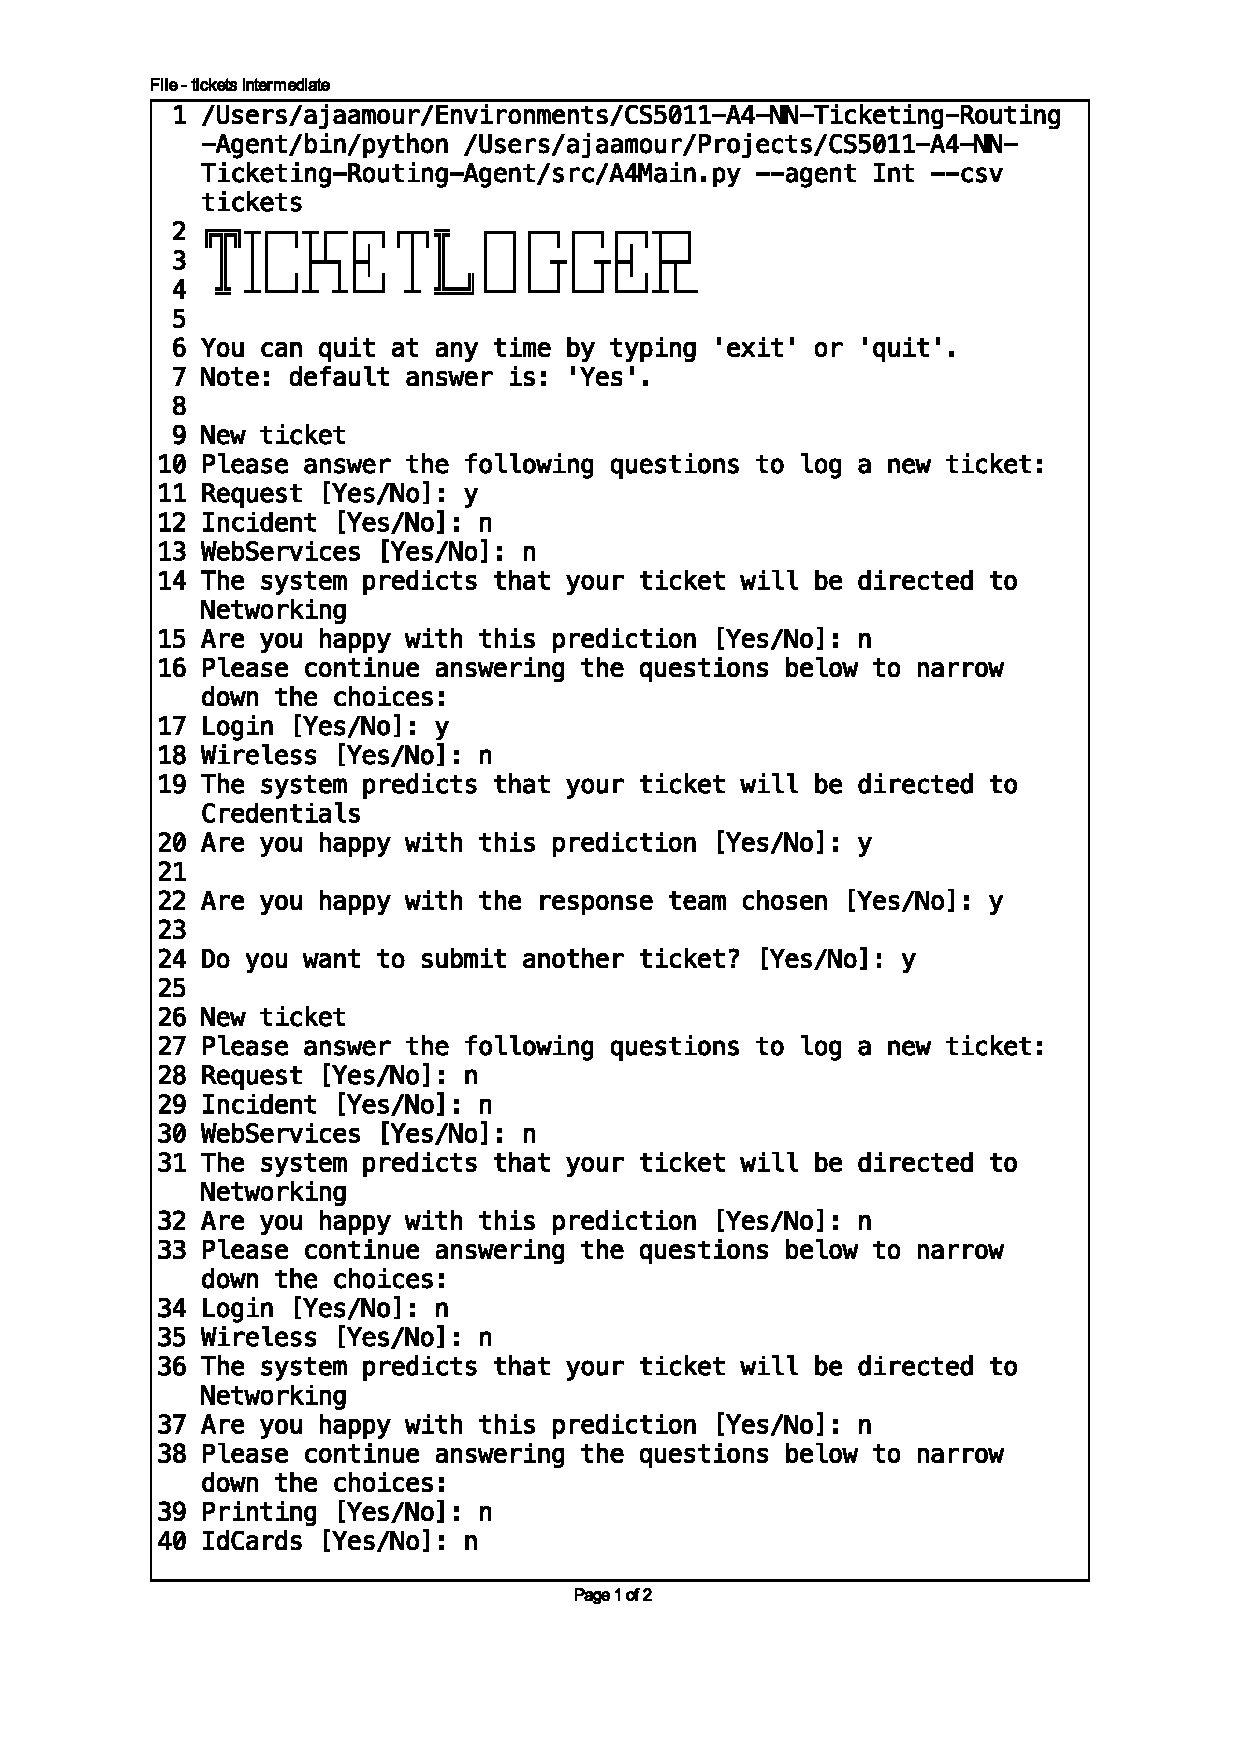
\includepdf[
    pages=1, 
    scale=0.8, 
    pagecommand=\section{Ticketing-Routing Agent Console Output Example}\label{sec:console-output-example}
]{figures/cli-output.pdf}
\includepdf[
    pages=2, 
    scale=0.8
]{figures/cli-output.pdf}

% ------------------------

\end{appendices}
\end{document}